\chapter{Experimentación y Resultados}\label{cap5}
\section{Infraestructura utilizada}

\subsection{Simulación de Red}

En un principio se hicieron experimentos utilizando software 
de simulación de redes para poder lograr tamaños de 
\emph{anonymity-set} aceptables. Este software utilizado fue 
\emph{CORE}\footnote{\url{https://www.nrl.navy.mil/itd/ncs/products/core}} 
el cual permite emular distintos nodos en una red simulada 
con los parámetros que el usuario estime convenientes. Utilizando 
este software se simularon nodos conectados a través de una red local, 
donde cada uno de los nodos se comporta como un participante dentro 
del protocolo anteriormente descrito.

Además de dicho software, se levantaron instancias de 
\emph{Docker}\footnote{\url{https://www.docker.com/}}, pudiendo así 
formar una red local entre los distintos contenedores corriendo 
en una misma máquina.

Ambas simulaciones mostraron un pobre rendimiento a la hora de 
correr el protocolo, mostrando tiempos de un orden de magnitud 
mayores que los tiempos reales que se lograron \emph{a posteriori}.

\subsection{Uso de red real}

Luego de notar los pobres resultados obtenidos en las simulaciones, se 
pudo obtener acceso a equipos reales conectados a través de una red 
local. En particular se utilizó el laboratorio \emph{Lorenzo} del 
Departamento de Ciencias de la Computación de la Universidad de Chile, el 
cual cuenta con 31 computadores, cantidad razonable para poder realizar 
las pruebas correspondientes.

\section{Experimentos Realizados}

Las pruebas realizadas fueron dos:

\begin{enumerate}
	\item Tamaño de sala variable, todos los participantes enviando: se 
	varió el tamaño de la sala desde 3 hasta 30 participantes, donde en 
	cada repetición, todos los participantes presentes envían un 
	mensaje de largo 140 caracteres.
	\item Tamaño de sala fijo, algunos participantes enviando: se fijó 
	el tamaño de la sala en 30 participantes, y en cada repetición se 
	aumentaba el número de mensajes (cada uno de 140 caracteres) enviados, 
	desde 1 hasta 30.
\end{enumerate}

En cada una de las dos pruebas realizadas se midieron los siguientes 
parámetros:

\begin{itemize}
	\item Tiempos de ejecución: se midieron tres distintos tiempos, (1) tiempo 
	total de la sesión, (2) tiempo que demora en llegar el primer mensaje, y 
	(3) tiempo promedio por ronda.
	\item \emph{Profiling} de cada etapa del protocolo: se midió que porcentaje 
	del tiempo total se gasta en cada una de las etapas del protocolo, en particular 
	cuanto tiempo se ocupa en etapas de procesamiento, y cuanto tiempo se ocupa 
	en etapas de comunicación.
	\item \emph{Overhead} resultante: al finalizar cada sesión, se midió el tamaño 
	del mensaje a enviar,y se dividió por la cantidad de tiempo que 
	duró la misma sesión, obteniendo así el \emph{overhead} necesario que añade
	el protocolo para proporcionar anonimato en el envío de mensajes.
\end{itemize}

\section{Resultados}

\subsection{Tiempos de Ejecución}

\begin{figure}[H]
  \centering
    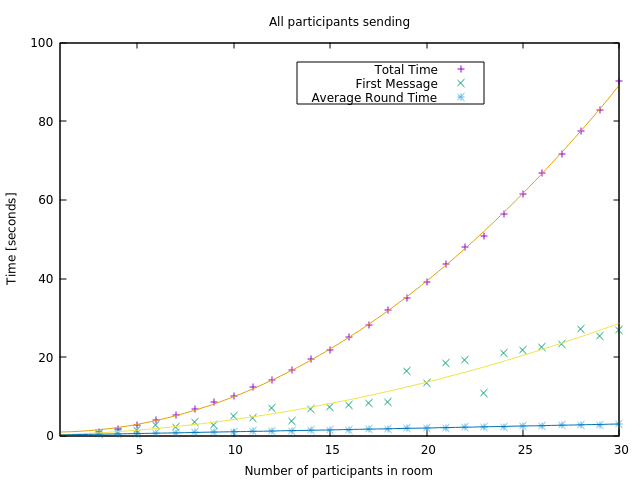
\includegraphics[scale=0.7]{logs/logs_all/times.png}
  \caption{Tiempos de Ejecución en Tamaño de sala variable}
  \label{fig:times-variable}
\end{figure}

\begin{figure}[H]
  \centering
    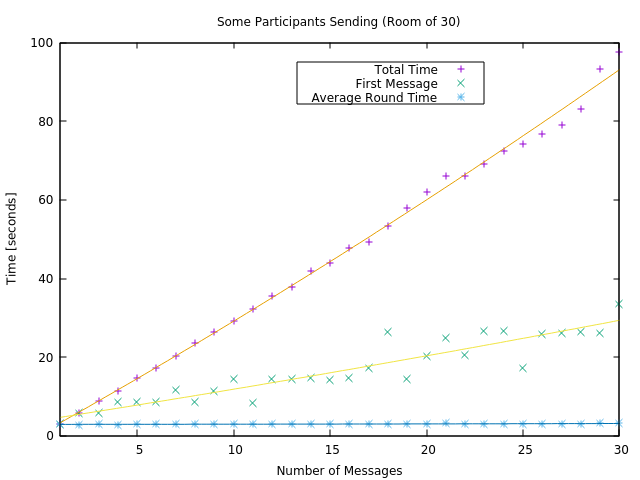
\includegraphics[scale=0.7]{logs/logs_partial_30/times.png}
  \caption{Tiempos de Ejecución en Tamaño de sala fijo}
  \label{fig:times-fixed}
\end{figure}

\subsection{\emph{Profiling} de las etapas}

\begin{figure}[H]
  \centering
    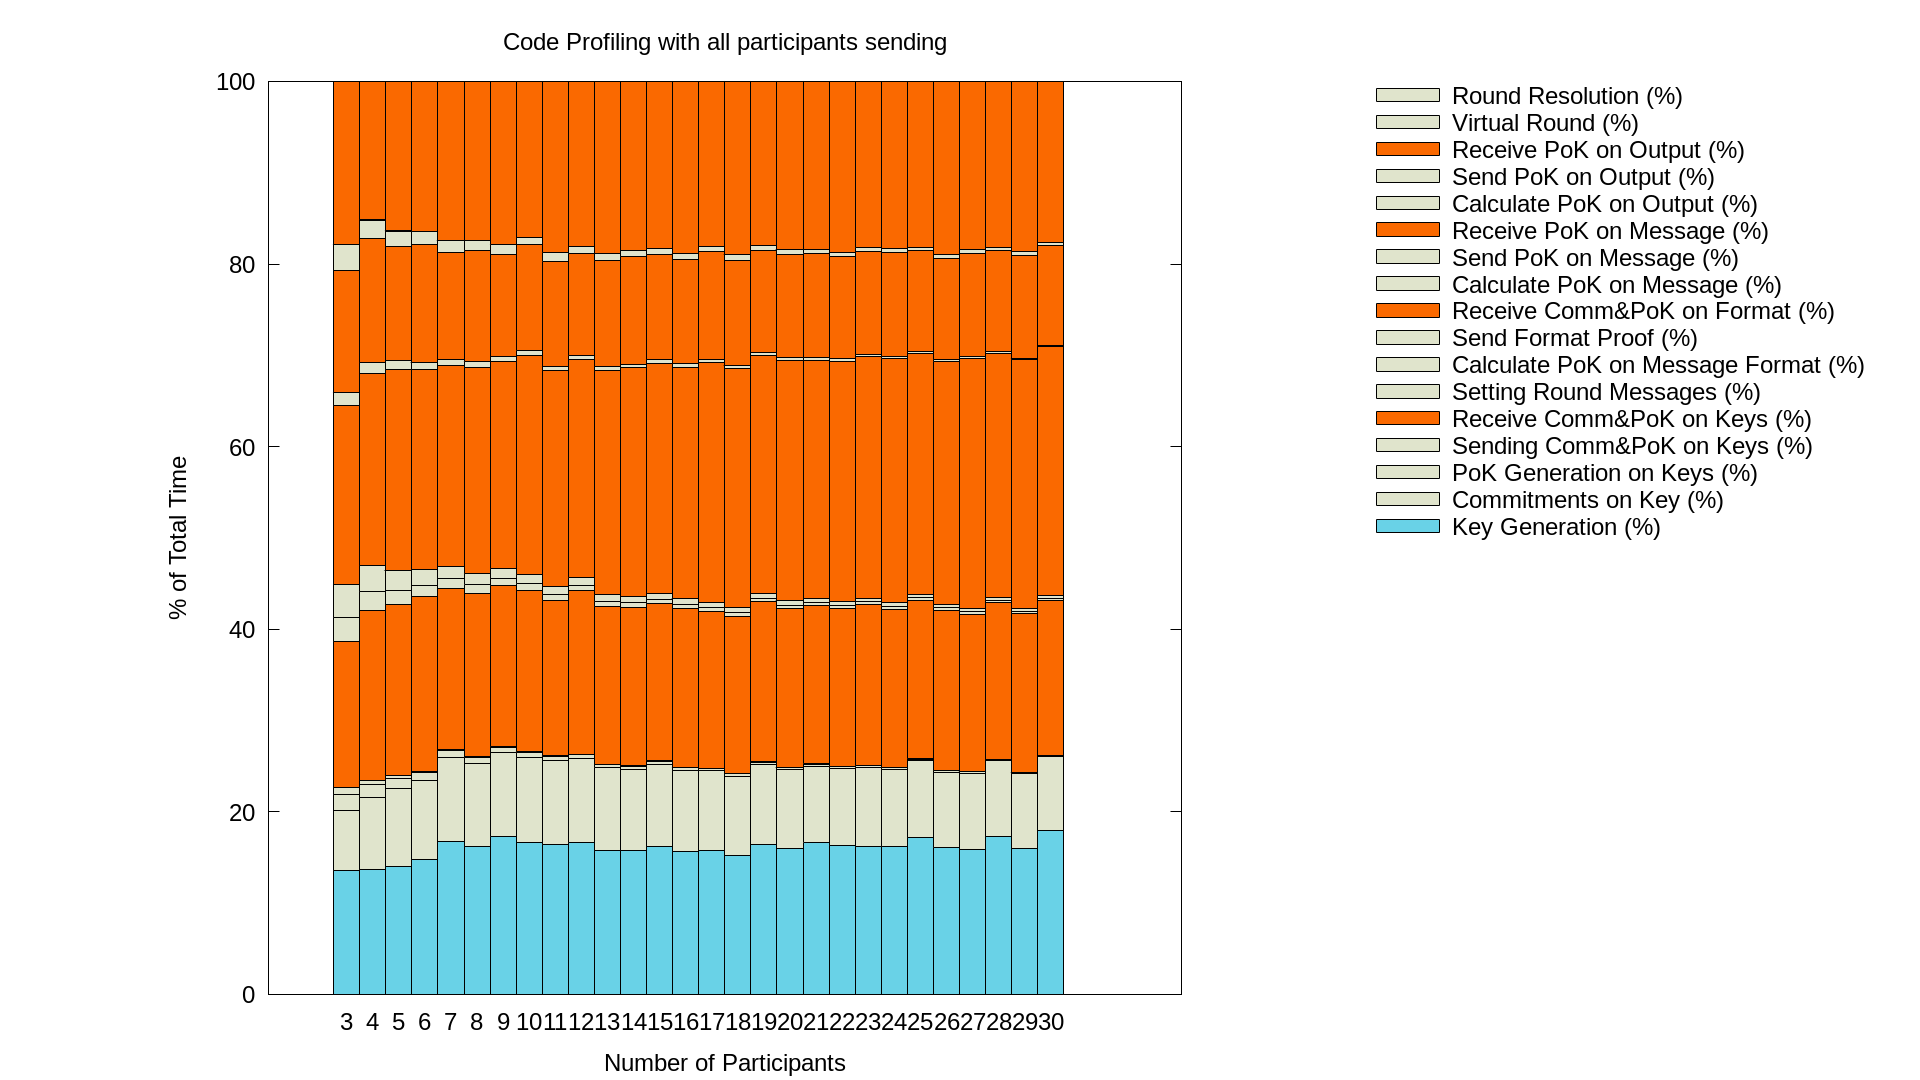
\includegraphics[scale=0.25]{logs/logs_all/profile.png}
  \caption{\emph{Profiling} de etapas en Tamaño de sala variable}
  \label{fig:profile-variable}
\end{figure}

\begin{figure}[H]
  \centering
    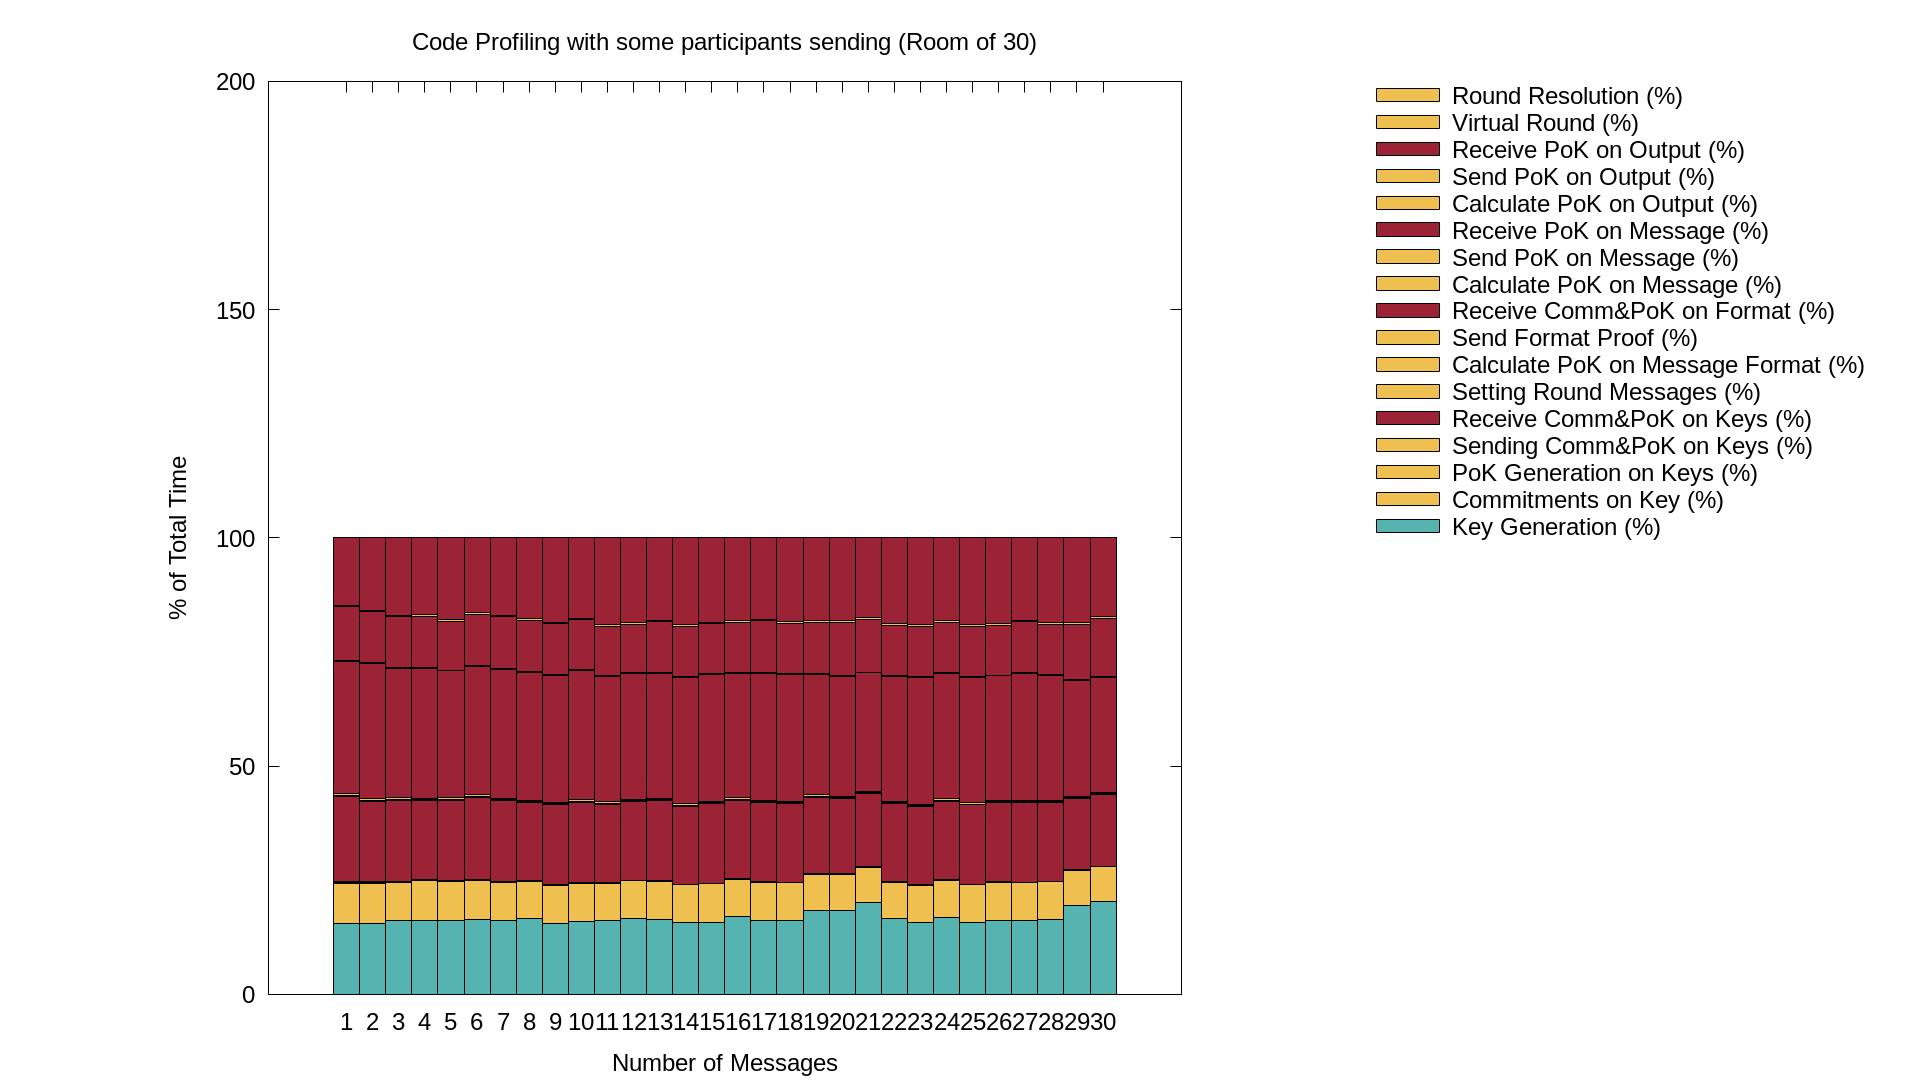
\includegraphics[scale=0.25]{logs/logs_partial_30/profile.png}
  \caption{\emph{Profiling} de etapas en Tamaño de sala fijo}
  \label{fig:profile-fixed}
\end{figure}

\subsection{\emph{Overhead} del protocolo}

\begin{figure}[H]
  \centering
    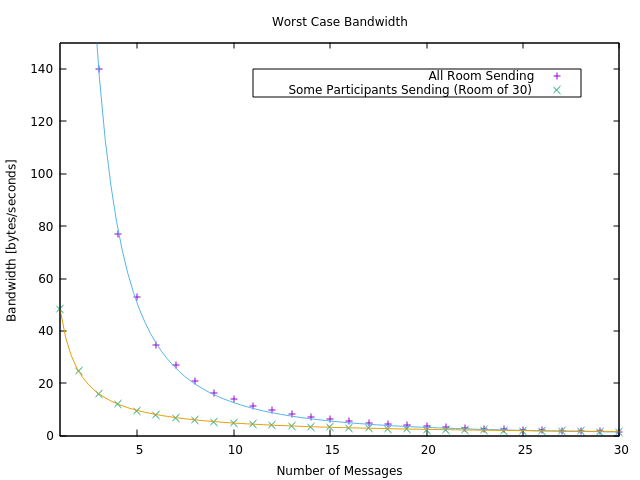
\includegraphics[scale=0.7]{logs/bandwidth.png}
  \caption{\emph{Bandwidth} del peor caso (último mensaje transmitido)}
  \label{fig:times-variable}
\end{figure}

\section{Discusión de los Resultados}

Las pruebas realizadas muestran varias tendencias que son dificiles de predecir 
solamente con la descripción teórica del protocolo criptográfico, mientras que otras 
son confirmaciones de resultados esperados observando netamente el diseño del 
protocolo.

Los puntos más importante a destacar son los siguientes:

\begin{itemize}
	\item Tiempos totales de ejecución: los tiempos totales de ejecución mostraron 
	resultados alentadores con relación al tiempo necesario que hay que esperar para 
	recibir mensajes de manera anónima. En el peor caso del experimento (30 mensajes 
	colisionando en una sala de 30 participantes), el tiempo total resultó ser de 
	1 minuto y 30 segundos, tiempo razonable para leer 30 mensajes de 140 caracteres 
	cada uno. Además importante notar que los primeros mensajes empiezan a llegar 
	aproximadamente a los 30 segundos de ejecución (en el mismo caso anterior), por lo que 
	hay una retroalimentación temprana que el protocolo está funcionando y empezando a 
	revelar los mensajes enviados.
	\item Tendencia en el aumento de tiempos: los tiempos totales muestran tendencias 
	que eran esperadas. Mientras que en la Figura \ref{fig:times-variable} los tiempos 
	totales siguen una tendencia cuadrática, esperada por el hecho que al agregar 
	un participante más al a sala, se elevan al cuadrado la cantidad de conexiones 
	necesarias (grafo totalmente conectado); en cambio en la Figura \ref{fig:times-fixed} los
	tiempos totales siguen una recta, mostrando que al fijar un tamaño de sala (en este caso, 
	30 participantes), el tiempo promedio por ronda se mantiene constante, independiente 
	del número de rondas necesarias para resolver la colisión, resultando así en una 
	tendencia lineal a medida que más mensajes colisionan en la primera ronda.
	\item Predominancia de las etapas de comunicación: el \emph{profiling} realizado, tanto 
	en el caso de tamaño de sala variable o fijo, muestra una predominancia abrumadora 
	de las etapas que implican un alto costo en la capa de comunicación (recepción de 
	\emph{commitments} y \emph{zero-knowledge proofs} enviados por otros participantes). 
	Independiente del tamaño de la sala o el número de mensajes involucrados en la colisión, 
	el tiempo de procesamiento (generación de \emph{commitments} y de \emph{zero-knowldge proofs}, 
	ejecutar una ronda virtual o procesar la resolución de la ronda), es significativamente 
	menor que las etapas de comunicación, por lo que mejoras al protocolo criptográfico en 
	términos de eficiencia (hacer \emph{zero-knowledge proofs} menos complejas, por ejemplo), no 
	significarían un incremento muy importante en el tiempo total de la ejecución del protocolo, 
	por lo que el trabajo futuro debería enfocarse en mejorar el rendimiento de la capa 
	de comunicación, manejando de manera más eficiente el envío y recepción de mensajes en la sala.
	\item Mejora al eliminar compartición de llaves: una propuesta sugerida en el \emph{paper} 
	original de la variante descrita en este trabajo \cite{franck2014dining}, hace referencia 
	a la eliminación de la etapa de compartición de llaves, e intercambiarla por una generación 
	pseudo aleatorio de la llave, compartiendo una semilla de generación entre cada par de participantes. 
	Las pruebas muestran que esta etapa se lleva entre un 10 y un 20 por ciento del tiempo total, 
	por lo que su eliminación mostraría una mejora importante en los tiempos totales de 
	ejecución del protocolo. 
	\item Costo extra para asegurar anonimato: alcanzar el nivel de anonimato que ofrece 
	el protocolo significa un sobre costo importante que cada participante debe pagar, reflejado 
	especialmente en la cantidad de información extra que debe enviarse con respecto al mensaje 
	final que desea comunicar. Estos tamaños se ven reflejados en la Tabla \ref{table:message_sizes_table}, 
	lo que muestra un altísimo sobre costo relativo que experimenta cada participante (alrededor de 
	70 veces por ronda y por participante presente en la sala). Eso quiere decir que si un participante 
	desea comunicar un mensaje de 140 caracteres en una sala de 30 participantes (y tiene la ``mala'' suerte 
	que todo el resto de la sala también quiere comunicar un mensaje), tendrá que enviar un 
	total de 8.8 MB de información aproximadamente. Junto con esto, en el peor caso (es decir, cuando 
	su mensaje es el último en ser revelado), experimentará un ancho de banda real de 1.5 bytes/sec 
	(para comunicar su mensaje de 140 bytes, tuvo que esperar 90 segundos). Esto presenta 
	un desafío muy importante a analizar por parte del diseño del protocolo criptográfico: ¿es 
	posible alcanzar el mismo nivel de anonimato, utilizando menos cantidad de mensajes? 
	¿pudieran acortarse las rondas o utilizar \emph{zero-knowledge proofs} más ``cortas''? 
	También es un desafío el mejorar la implementación y tratar de disminuir la cantidad de información 
	enviada a través de la red, por ejemplo a través de mecanismos de compresión de información, pero 
	procurando que los tiempos necesarios para comprimir y descomprimir la información sean tales 
	que se evidencie una mejora sustancial en los tiempos totales de la ejecución del protocolo.
\end{itemize}

\subsection{Escenario propuesto de uso}

Con los resultados discutidos anteriormente, se propone un escenario que logre 
porporcionar anonimato a sus participantes, y que esto no suponga pagar un alto 
costo por un rendimiento pobre de la aplicación desarrollada.

Como el protocolo es altamente sensible a (1) el tamaño de los mensajes, y (2) cantidad 
de mensajes colisionando, se propone utilizar la aplicación implementada en un contexto 
de \emph{microblogging}, con una creación de sesiones de manera periódica, otorgando 
así la posibilidad de mantener un tamaño del \emph{anonimity-set} considerable y reducir 
la posibilidad de colisiones masivas de mensajes, para así poseer un envío de mensajes 
más eficiente.

Una posible configuración del escenario anterior es el siguiente: creación de una sala 
de 30 participantes, los cuales participan cada 30 minutos en la ejecución de una sesión, 
cada uno contribuyendo para el normal desarrollo del protocolo, mientras que una fracción 
de ellos va a tener la necesidad de enviar un mensaje (de un máximo de 140 caracteres, 
\emph{á la} Twitter) en la sesión actual. Al tener una repetición periódica de la ejecución 
de sesiones, la posibilidad de una colisión masiva de mensajes en cada una de ellas es menor, 
logrando así que cada una de ellas pueda resolver de manera rápida la colisión de los mensajes 
resultantes, logrando así que cada participante que necesite enviar un mensaje, observe una 
baja latencia y pueda comunicarse de manera rápida y expedita. La ejecución de sesiones 
debe hacerse de manera constante, teniendo que en muchas de ellas no se enviará ningún mensaje, 
resultando así en una ejecución rápida y de bajo costo para todos los participantes. Además de esta 
manera se pueden agregar o expulsar a participantes entre sesiones, para así, ya sea aumentar 
el anonimato, o bien castigar a participantes que se comportaron de manera maliciosa en sesiones 
anteriores (la ejecución de las sesiones es totalmente independiente unas de otras).

El escenario anterior podría instanciarse en varios contextos donde se necesita la opción 
de comunicar mensajes de manera anónima:
\begin{itemize}
	\item Denuncias de abusos laborales dentro de una corporación privada.
	\item Foro de denunciantes (\emph{whistleblowers}) de actividades 
	realizadas por alguna institución pública.
	\item Foro de conversación entre distintos centros periodisticos (al poseer mayor 
	poder de cómputo, se puede permitir el envío de mensajes de mayor longitud).
	\item Votaciones secretas periódicas entre un grupo de interés (en vez de enviar un mensaje, 
	simplemente se envía un bit, diferenciando entre SI y NO).
\end{itemize} 